\documentclass[../../main.tex]{subfiles}
\begin{document}

{\bf [解]}

与えられた方程式$e^{x}-x^{e}=k$の正の解の個数は，$xy$平面上の二つのグラフ
\begin{align}
 \begin{cases}
   y = f(x) = e^x-x^e & (x>0) \\
   y = k
 \end{cases} \label{eq:1}
\end{align}
の交点の数に等しい．そこで$y=f(x)$の挙動を調べよう．
一階微分は
\begin{align}
 f'(x)=e^x-e\cdot x^{e-1}
\end{align}
だから$x>0$の時
\begin{align}
 &f'(x)\ge 0 \\
\iff 
 &e^x\ge e\cdot x^{e-1} \\
\iff
 &x\ge 1+(e-1)\log x \\
 &x-1-(e-1)\log x \ge 0 \label{eq:2}
\end{align}
である．ただし最後は両辺の自然対数をとった．ここで\cref{eq:2}の左辺を$g(x)$とおく：
\begin{align}
 g(x)=x-1-(e-1)\log x
\end{align}
と一階微分は
\begin{align}
 g'(x)=1-\dfrac{e-1}{x}
\end{align}
だから$g(x)$の増減表は以下のようになる．ただし，$g(x)=0$の解は
\begin{align}
 \begin{cases}
  g(1)=1-1-(e-1)\log1=0 \\
  g(e)=e-1-(e-1)\log e=e-1-(e-1)=0
 \end{cases}
\end{align}
の二つがあることを用いた．増減表からこれ以外の解は存在しない．

\begin{table}[htb]
\centering
\caption{$g(x)$ の増減表}
\begin{tabular}{c|cccccccc}
$x$ & $(0)$ & $\cdots$ & $1$ & $\cdots$ & $e-1$ & $\cdots$ & $e$ & $\cdots$ \\
\hline
$g'(x)$ & & $-$ & $-$ & $-$ & $0$ & $+$ & $+$ & $+$ \\
\hline
$g(x)$ & & $\searrow$ & $0$ & $\searrow$ & 極小 & $\nearrow$ & $0$ & $\nearrow$
\end{tabular}
\end{table}

従って，\cref{eq:2}から$f'(x) \ge 0$となるのは$0<x \le 1, e\le x$の時で，$f(x)$の増減表は以下のようになる．

\begin{table}[htb]
\centering
\caption{$f(x)$ の増減表}
\begin{tabular}{c|ccccccc}
$x$ & $(0)$ & $\cdots$ & $1$ & $\cdots$ & $e$ & $\cdots$ \\
\hline
$f'(x)$ & & $+$ & $0$ & $-$ & $0$ & $+$ \\
\hline
$f(x)$ & $(1)$ & $\nearrow$ & $e-1$ & $\searrow$ & $0$ & $\nearrow$
\end{tabular}
\end{table}

よって$y=f(x)$のグラフの形状は以下のようになる．

\begin{figure}[htb]
\centering
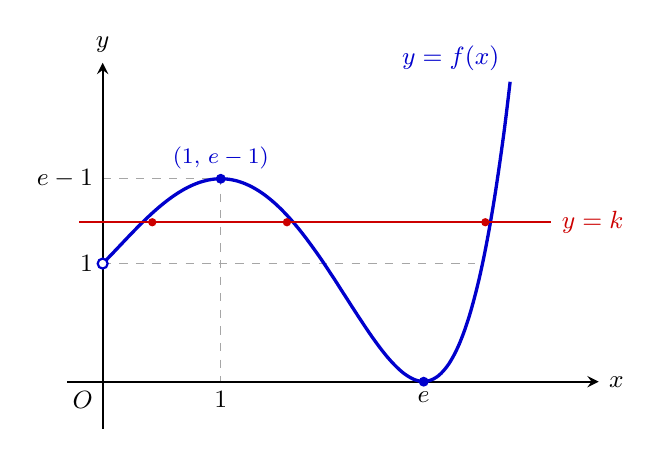
\begin{tikzpicture}[scale=1.5, >=stealth, every node/.style={font=\small}]

  % 1. 補助線（点線）
  % y = e-1 (極大値 y \approx 1.718)
  \draw[dashed, gray!70] (0, 1.718) -- (1.0, 1.718) -- (1.0, 0);
  % y = 1 (x -> +0 での極限)
  \draw[dashed, gray!70] (0, 1.0) -- (3.15, 1.0);
  % x = e (極小点 x \approx 2.718)
  \draw[dashed, gray!70] (2.718, 0) -- (2.718, 0);

  % 2. 座標軸
  \draw[->, thick] (-0.3, 0) -- (4.2, 0) node[right] {$x$};
  \draw[->, thick] (0, -0.4) -- (0, 2.7) node[above] {$y$};
  \node[below left] at (0,0) {$O$};

  % 3. y = f(x) = e^x - x^e の曲線描画
  % (0, 1) から極大 (1, e-1) を経て極小 (e, 0) へ、その後急上昇
  \draw[domain=0.03:3.45, smooth, very thick, blue!80!black, samples=80] 
    plot (\x, {exp(\x) - (\x)^2.71828}) node[above left] {$y = f(x)$};

  % 4. 直線 y = k の代表例（1 < k < e-1: 3交点）
  \draw[thick, red!80!black] (-0.2, 1.35) -- (3.8, 1.35) node[right] {$y = k$};

  % 5. 軸上の目盛りラベル
  \node[left] at (0, 1.0) {$1$};
  \node[left] at (0, 1.718) {$e-1$};
  \node[below] at (1.0, 0) {$1$};
  \node[below] at (2.718, 0) {$e$};

  % 6. プロット点
  % x -> +0 の除外点 (0, 1) : 白抜き丸
  \fill[white] (0, 1.0) circle (1.2pt);
  \draw[thick, blue!80!black] (0, 1.0) circle (1.2pt);

  % 極大点 (1, e-1)
  \fill[blue!80!black] (1.0, 1.718) circle (1.2pt) 
    node[above] {\footnotesize $(1,\, e-1)$};

  % 極小点 (e, 0)
  \fill[blue!80!black] (2.718, 0) circle (1.2pt);

  % 3つの交点プロット (y = k との交点)
  \fill[red!80!black] (0.42, 1.35) circle (1.0pt);
  \fill[red!80!black] (1.56, 1.35) circle (1.0pt);
  \fill[red!80!black] (3.24, 1.35) circle (1.0pt);

\end{tikzpicture}
\caption{$y=f(x)$ のグラフと直線 $y=k$ の交点}
\end{figure}



グラフから$y=k$との交点の個数（$=$求める解の個数）は次のようになる：
\begin{align}
\begin{cases}\displaystyle
0\text{個} & (k<0)\\
1\text{個} & (k=0)\\
2\text{個} & (0<k\le1)\\
3\text{個} & (1<k<e-1)\\
2\text{個} & (k=e-1)\\
1\text{個} & (k>e-1)
\end{cases}
\end{align}


\newpage

\end{document}
